% Copyright 2011-2014 David Hadka.  All Rights Reserved.
%
% This file is part of the MOEA Framework User Manual.
%
% Permission is granted to copy, distribute and/or modify this document under
% the terms of the GNU Free Documentation License, Version 1.3 or any later
% version published by the Free Software Foundation; with the Invariant Section
% being the section entitled "Preface", no Front-Cover Texts, and no Back-Cover
% Texts.  A copy of the license is included in the section entitled "GNU Free
% Documentation License".

\chapter{Installation Instructions}

This chapter details the steps necessary to download and install the MOEA Framework on your computer.

\section{Understanding the License}

Prior to downloading, using, modifying or distributing the MOEA Framework, developers should make themselves aware of the conditions of the GNU Lesser General Public License (GNU LGPL).  While the GNU LGPL is a free software license, it does define certain conditions that must be followed in order to use, modify and distribute the MOEA Framework library.  These conditions are enacted to ensure that all recipients of the MOEA Framework (in its original and modified forms) are granted the freedoms to use, modify, study and distribute the MOEA Framework so long as the conditions of the GNU LGPL are met.  Visit \webpage{http://www.gnu.org/licenses/lgpl.html} to read the full terms of this license.

\section{Which Distribution is Right for Me?}

The MOEA Framework is currently distributed in three forms: 1) the compiled binaries; 2) the all-in-one executable JAR file; and 3) the source code.  The following text describes each distribution and its intended audience.

\paragraph{Compiled Binaries}
The compiled binaries distribution contains a fully-working MOEA Framework installation.  All required third-party libraries, data files and documentation are provided.  This download is recommended for developers integrating the MOEA Framework into an existing project.

\paragraph{All-in-One Executable}
The all-in-one executable distribution is similar to the compiled binaries.  It provides a fully-working MOEA Framework installation with one major difference: all files are packaged into a single JAR file.  This distribution is intended for first-time users and, in particular, for demonstrating the MOEA Diagnostic Tool by double-clicking the JAR file.

\paragraph{Source Code}
The source code distribution contains all source code, unit tests, documentation and data files.  This distribution gives users full control over the MOEA Framework, as any component can be modified as needed.  As such, this download is recommended for developers wishing to contribute to or study the inner workings of the MOEA Framework.

\section{Obtaining a Copy}

The various MOEA Framework distributions can be downloaded from our website at \webpage{http://www.moeaframework.org/}.  The compiled binaries and source code distributions are packaged in a compressed tar (.tar.gz) file.  Unix/Linux/Mac users can extract the file contents using the following command:

\begin{lstlisting}[language=Plaintext]
tar -xzf MOEAFramework-%VERSION%.tar.gz
\end{lstlisting}

Windows users must use an unzip utility like 7-Zip to extract the file contents.  7-Zip is a free, open source program which can be downloaded from \webpage{http://www.7-zip.org/}.

\section{Installing Dependencies}

The software packages listed below are required or recommended in order to use the MOEA Framework.  Any software package marked as required MUST be installed on your computer in order to use the MOEA Framework.  Software marked as optional is not required to be installed, but will generally make your life easier.  This manual will often provide instructions specific to these optional software packages.

\subsection{Java 6+ (Required)}
Java 6, or any later version, is required for any system running the MOEA Framework.  If downloading the compiled binaries or all-in-one executable, you only need to install the Java Runtime Environment (JRE).  The source code download requires the Java Development Kit (JDK), which contains the compiler and other developer tools.  We recommend one of the following vendors (most are free):

\begin{description}
  \item[Oracle] - \webpage{http://www.oracle.com/technetwork/java/javase/}
    \begin{itemize}
      \item For Windows, Linux and Solaris
    \end{itemize}
    
  \item[JRockit JDK] - \webpage{http://www.oracle.com/technetwork/middleware/jrockit/}
    \begin{itemize}
      \item For Windows, Linux and Solaris
      \item May provide better performance and scalability on Intel 32 and 64-bit architectures
    \end{itemize}

  \item[OpenJDK] - \webpage{http://openjdk.java.net/}
    \begin{itemize}
      \item For Ubuntu 8.04 (or later), Fedora 9 (or later), Red Hat Enterprise Linux 5, openSUSE 11.1, Debian GNU/Linux 5.0 and OpenSolaris
    \end{itemize}

  \item[IBM] - \webpage{http://www.ibm.com/developerworks/java/jdk/}
    \begin{itemize}
      \item For AIX, Linux and z/OS
    \end{itemize}
  \item[Apple] - \webpage{http://support.apple.com/kb/DL1572}
\end{description}

Please follow the installation instruction accompanying your chosen JRE or JDK.

\subsection{Eclipse or NetBeans (Optional)}
Eclipse and NetBeans are two development environments for writing, debugging, testing, and running Java programs.  Eclipse can be downloaded for free from \webpage{http://www.eclipse.org/}, and NetBeans can be obtained from \webpage{http://netbeans.org/}.

The installation of Eclipse is simple --- just extract the compressed file to a folder of your choice and run the Eclipse executable from this folder.  First-time users of Eclipse may be prompted to select a workspace location.  The default location is typically fine.  Click the checkbox to no longer show this dialog and click Ok.

To install NetBeans, simply run the executable.  Once installed, you can launch NetBeans by clicking the NetBeans link in your start menu.

\subsection{Apache Ant (Optional)}
Apache Ant is a Java tool for automatically compiling and packaging projects, similar to the Make utility on Unix/Linux.  Individuals working with the source code distribution should consider installing Apache Ant, as it helps automate building and testing the MOEA Framework.  Apache Ant can be downloaded from \webpage{http://ant.apache.org/}.  The installation instructions provided by Ant should be followed.

Note that Eclipse contains Ant, so it is not necessary to install Eclipse and Ant together.

\section{Importing into Eclipse}
When working with the source code distribution, it is necessary to properly configure the Java environment to ensure all resources are available.  To assist in this process, the source code distribution includes the necessary files to import directly into Eclipse.

To import the MOEA Framework project into Eclipse, first start Eclipse and select File $\rightarrow$ Import... from the menu.  A popup window will appear.  Ensure the General $\rightarrow$ Existing Projects into Workspace item is selected and click Next.  A new window will appear.  In this new window, locate the Set Root Directory entry.  Using the Browse button, select the \folder{\moeaframework} folder containing the source code.  Finally, click Finish.  The MOEA Framework will now be properly configured in Eclipse.

\section{Importing into NetBeans}
If you downloaded the source code, you can import the MOEA Framework into NetBeans as follows.  In NetBeans, select New Project from the File menu.  In the screen that appears, select the ``Java'' category and ``Java Project with Existing Sources''.  Click Next.

Specify the project name as ``MOEA Framework''.  Set the project folder by clicking the Browse button and selecting the \folder{\moeaframework} folder.  Click Next.

Add the \folder{src} and \folder{examples} folders as Source Package Folders.  Click Finish.  The MOEA Framework project should now appear in the Projects window.

Finally, we need to add the third-party libraries used by the MOEA Framework.  Right-click the MOEA Framework project in the Projects window and select Properties.  In the window that appears, click Libraries in the left-hand panel.  On the right-side of the window, click the button ``Add Jars/Folder''.  Browse to the \folder{\moeaframework/lib} folder, highlight all the JAR files (using shift or alt to select multiple files), and click Ok.  Be sure that you select each individual JAR file and not the folder containing the JAR files.  Click the ``Add Jars/Folder'' button again.  Navigate to and select the root \folder{\moeaframework} folder, and click Ok.  You should now see $8$ items in the compile-time libraries list.  There should be $7$ entries referencing \plaintext{.jar} files the ``\folder{.}'' as the last entry.  Your screen should look like \figref{fig:netbeans}.  Click Ok when finished.

\begin{figure}
  \center
  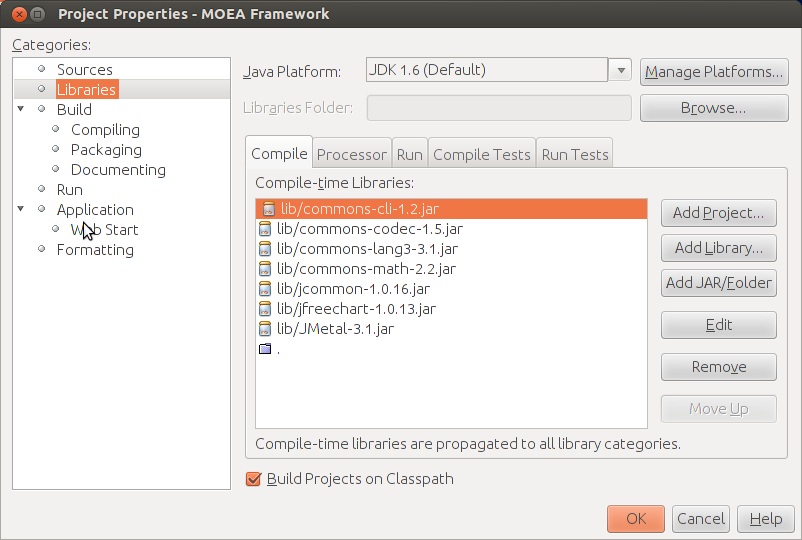
\includegraphics[width=.8\linewidth]{netbeans.png}
  \caption{How the NetBeans properties window should appear in the MOEA Framework is properly configured.}
  \label{fig:netbeans}
\end{figure}

\begin{important}
Test your NetBeans install by running Example1.  You can run an example by expanding the \folder{examples} folder in the Project window, right-clicking Example1, and selecting Run File from the popup menu.  If you receive a ``provider not found'' error, go back to the previous step and ensure the ``\folder{.}'' entry is listed as a compile-time library.  This is required for the Java Service Provider Interface (SPI) mechanism to properly locate algorithms and problems built into the MOEA Framework.
\end{important}

\section{Testing your Installation}
Having finished installing the MOEA Framework and its dependencies, it is useful to run the MOEA Diagnostic Tool to test if the installation was successful.  If the diagnostic tool appears and you can run any algorithm, then the installation was successful.

\paragraph{Compiled Binaries}
Run the launch-diagnostic-tool.bat file on Windows.  You can manually run the diagnostic tool with the following command:

\begin{lstlisting}[language=Plaintext]
java -Djava.ext.dirs=lib
		org.moeaframework.analysis.diagnostics.LaunchDiagnosticTool
\end{lstlisting}

\paragraph{All-in-One Executable}
Double-click the downloaded JAR file.  If the Diagnostic Tool window does not appear, try to manually launch the tool with with the following command:

\begin{lstlisting}[language=Plaintext]
java -jar MOEAFramework-%VERSION%-Executable.jar
\end{lstlisting}

\paragraph{Source Code}
Inside Eclipse, navigate to the src $\rightarrow$ org $\rightarrow$ moeaframework $\rightarrow$ analysis $\rightarrow$ diagnostic package in the Package Explorer window.  Right-click the file \texttt{LaunchDiagnosticTool.java} and select the Run as $\rightarrow$ Java Application option in the popup menu.

\section{Distribution Contents}
This section describes the contents of the compiled binaries and source code distribution downloads.

\subsection{Compiled Binary Contents}
\begin{description}
  \item[\folder{javadoc/}] contains the MOEA Framework API, which is a valuable resource for software developers as it provides descriptions of all classes, methods and variables available in the MOEA Framework.  The API may be viewed in a web browser by opening the \file{index.html} file.
  \item[\folder{lib/}] contains the compiled libraries required to use the MOEA Framework.  This includes the MOEA Framework compiled libraries and all required third-party libraries.
  \item[\folder{licenses/}] contains the complete text of all open source software licenses for the MOEA Framework and third-party libraries.  In order to comply with the licenses, this folder should always be distributed alongside the compiled libraries in the lib folder.
  \item[\folder{pf/}] contains the Pareto front files for the test problems provided by default in the MOEA Framework.
  \item[\file{global.properties}] is the configuration file for the MOEA Framework.  Default settings are used unless the settings are provided in this file.
  \item[\file{HELP}] provides a comprehensive list of errors and warning messages encountered when using the MOEA Framework.  When available, information about the cause and ways to fix errors are suggested.
  \item[\file{launch-diagnostic-tool.bat}] launches the diagnostic tool GUI that allows users to run algorithms and display runtime information about the algorithms.  This file is for Windows systems only.
  \item[\file{LICENSE}] lists the open source software licenses in use by the MOEA Framework, contributor code and third-party libraries.
  \item[\file{NEWS}] details all important changes made in the current release and prior releases.  This includes critical bug fixes, changes, enhancements and new features.
  \item[\file{README}] provides information about obtaining, installing, using, distributing, licensing and contributing to the MOEA Framework.
\end{description}

\subsection{Source Code Contents}
\begin{description}
  \item[\folder{auxiliary/}] contains an assortment of files and utilities used by the MOEA Framework, but are not required in a build.  For instance, this folder contains example C/C++ code for interfacing C/C++ problems with the MOEA Framework.
  \item[\folder{examples/}] contains examples using the MOEA Framework.  These examples are also available on the website.
  \item[\folder{lib/}] contains all required third-party libraries used by the MOEA Framework.
  \item[\folder{manual/}] contains the LaTeX files and figures for generating this user manual.
  \item[\folder{META-INF/}] contains important files which are packaged with the compiled binaries.  Such files include the service provider declarations, licensing information, etc.
  \item[\folder{pf/}] contains the Pareto front files for the test problems provided by default in the MOEA Framework.
  \item[\folder{src/}] contains all source code in use by the core MOEA Framework library.
  \item[\folder{test/}] contains all JUnit unit tests used to ensure the correctness of the MOEA Framework source code.
  \item[\folder{website/}] contains all files used to generate the website.
  \item[\file{build.xml}] contains the Apache Ant build scripts for compiling and/or building the MOEA Framework library.
  \item[\file{global.properties}] is the configuration file for the MOEA Framework.  Default settings are used unless the settings are provided in this file.
  \item[\file{HELP}] provides a comprehensive list of errors and warning messages encountered when using the MOEA Framework.  When available, information about the cause and ways to fix errors are suggested.
  \item[\file{LICENSE}] lists the open source software licenses in use by the MOEA Framework, contributor code and third-party libraries.
  \item[\file{NEWS}] details all important changes made in the current release and prior releases.  This includes critical bug fixes, changes, enhancements and new features.
  \item[\file{README}] provides information about obtaining, installing, using, distributing, licensing and contributing to the MOEA Framework.
  \item[\file{test.xml}] contains the Apache Ant testing scripts used to automatically run all JUnit unit tests and provide a human-readable report of the test results.
  \item[\file{TODO}] lists all planned changes for the MOEA Framework source code.  This file is a starting point for individuals wishing to contribute modifications to the MOEA Framework.
\end{description}

\section{Conclusion}
This chapter described each of the MOEA Framework distributions.  At this point, you should have a working MOEA Framework distribution which you can use to run the examples in subsequent chapters.